\subsubsection{UC\theuccount-GP - Accesso}
		\begin{figure}[H]
			\centering
				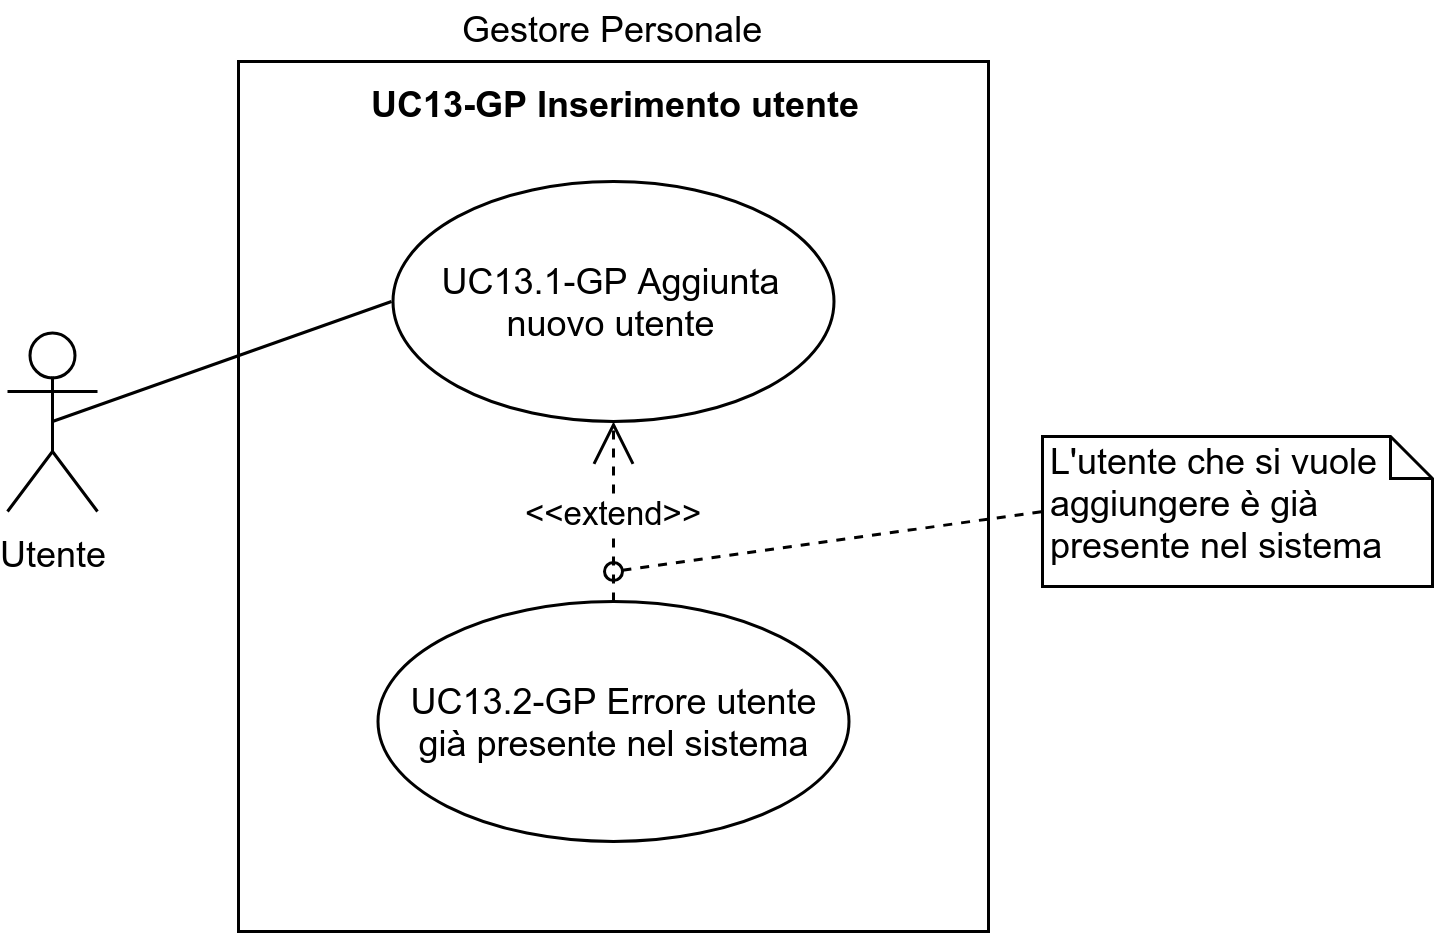
\includegraphics[width=0.8\textwidth]{img/casi_d'uso/UC13.png}\\
			\caption{UC\theuccount-GP - Accesso}
		\end{figure}
	\begin{itemize}
		\item \textbf{Codice}: UC\theuccount-GP.
		\item \textbf{Titolo}: accesso.
		\item \textbf{Attori primari}: utente non acceduto.
		\item \textbf{Descrizione}: l'utente non acceduto richiede di accedere al sistema attraverso l'inserimento dell'identificativo che viene creato nel momento della registrazione.
		\item \textbf{Precondizione}: il sistema considera l’utilizzatore come un utente non acceduto.
		\item \textbf{Postcondizione}: il sistema riconosce l'utilizzatore di esso come utente acceduto.
		\item \textbf{Scenario Principale}:
		\begin{enumerate}
			\item L'utente non ancora riconosciuto dal sistema procede all'accesso inserendo il proprio identificativo
		\end{enumerate}
	\end{itemize}
	
	\stepcounter{subuccount}
	\paragraph{UC\theuccount.\thesubuccount-GP - Accesso dell'utente nel sistema}
		\begin{figure}[H]
			\centering
				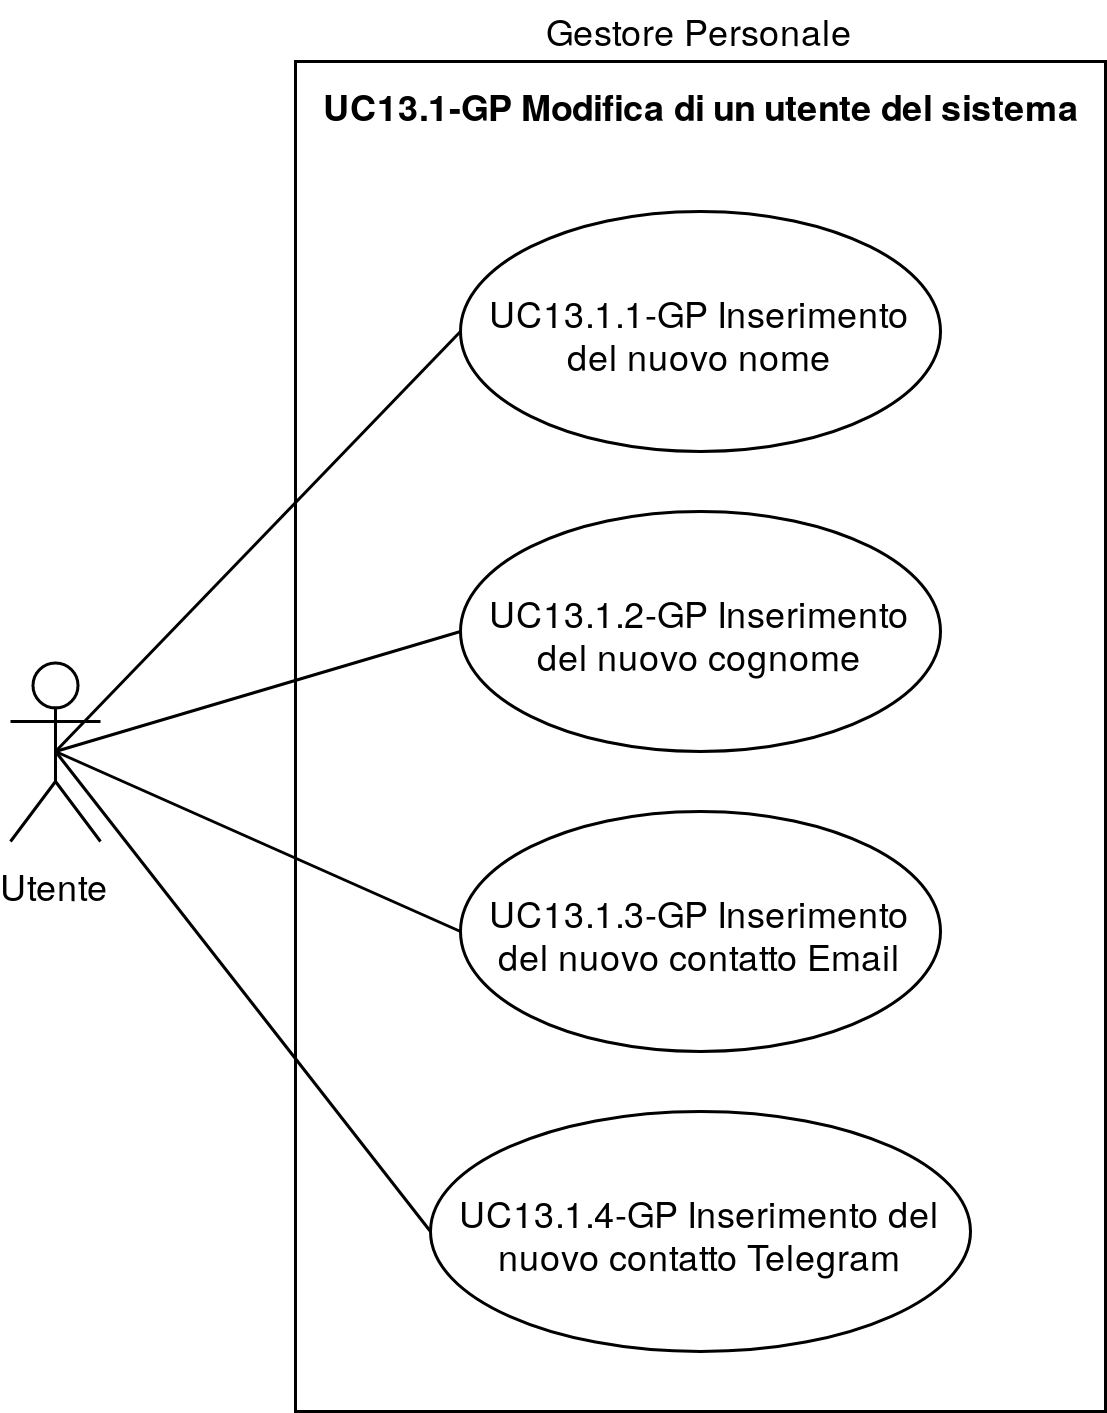
\includegraphics[width=0.5\textwidth]{img/casi_d'uso/UC13_1.png}\\
			\caption{UC\theuccount.\thesubuccount-GP - Accesso dell'utente nel sistema}
		\end{figure}
		\begin{itemize}
			\item \textbf{Codice}: UC\theuccount.\thesubuccount-GP.
			\item \textbf{Titolo}: accesso dell'utente nel sistema.
			\item \textbf{Attori primari}: utente non acceduto.
			\item \textbf{Descrizione}: l'utente attende l'accesso al sistema.
			\item \textbf{Precondizione}: il sistema riconosce l'utilizzatore come un utente non acceduto.
			\item \textbf{Postcondizione}: il sistema riconosce l'utente con successo.
			\item \textbf{Scenario Principale}:
			\begin{enumerate}
				\item L’utente non ancora riconosciuto dal sistema richiede l'accesso attraverso l'inserimento dell'identificativo.
			\end{enumerate}
			\item \textbf{Estensioni}:
			\begin{enumerate}
				\item L'accesso non va a buon fine e viene visualizzato un errore avvisando l'utente [UC\theuccount.2-GP]
			\end{enumerate}
		\end{itemize}
		
		\newpage
		
		\stepcounter{subsubuccount}
		\subparagraph{UC\theuccount.\thesubuccount.\thesubsubuccount-GP - Inserimento identificativo}
			\begin{itemize}
				\item \textbf{Codice}: UC\theuccount.1.1-GP.
				\item \textbf{Titolo}: inserimento identificativo.
				\item \textbf{Attori primari}: utente non acceduto.
				\item \textbf{Descrizione}: l'utente inserisce l'identificativo.
				\item \textbf{Precondizione}: il sistema riconosce l'utilizzatore come un utente non acceduto e permette all'utente l'inserimento dell'identificativo.
				\item \textbf{Postcondizione}: l'utente ha inserito l'identificativo desiderato.
				\item \textbf{Scenario Principale}:
				\begin{enumerate}
					\item L'utente inserisce l'identificativo per autenticarsi
				\end{enumerate}
			\end{itemize}
	
	\stepcounter{subuccount}
	\paragraph{UC\theuccount.\thesubuccount-GP - Errore identificativo inesistente}
		\begin{itemize}
			\item \textbf{Codice}: UC\theuccount.\thesubuccount-GP.
			\item \textbf{Titolo}: errore identificativo inesistente.
			\item \textbf{Attori primari}: utente non acceduto.
			\item \textbf{Descrizione}: l'utente viene avvisato che ha inserito un identificativo errato.
			\item \textbf{Precondizione}: il sistema riconosce l'utilizzatore come un utente non acceduto e riceve una richiesta di accesso. 
			\item \textbf{Postcondizione}: il sistema comunica all'utilizzatore l'errore.
			\item \textbf{Scenario Principale}:
			\begin{enumerate}
				\item L'utente inserisce un identificativo non esistente
				\item L'utente visualizza il messaggio d'errore
			\end{enumerate}
		\end{itemize}
